\section{Thesis Project Plan}
\label{sec:thesis}

The main goal of this thesis is to find an approximate solution to The Art Gallery Problem \cite{o1987art} using gradient descent. As such, we will devise an algorithm for optimising the positions of the guards inside the given Art Gallery polygon. 
The algorithm will be coded in C ++ with the help of the CGAL library(\url{https://www.cgal.org}).

\subsection{Motivation}
% see what Till says

\subsection{Progress So Far}
The first four weeks of the project have been spent on doing literature research.

Two weeks have been spent on creating the C ++ skeleton and trying out already given examples.

The rest of the time has been spent on devising the gradient computation for one guard and implementing it.
The pseudo-code can be found in Algorithm \ref{alg:1g}.

\begin{algorithm}
    \begin{algorithmic}[1]
    \caption{Position Optimisation for One Guard}
    \label{alg:1g}
    \For{\textbf{each} guard $p(x, y)$}
        \State{\textit{cur\_guard\_position} $\gets (x, y)$}

        \While{\textit{prev\_guard\_position} $\neq$ \textit{cur\_guard\_position}} \Comment{continue as long as there are no more improvements in the guard's position}
            % \State{compute \textit{visibility\_region} of $p$}
            \State{compute $\bigtriangledown f$}
            \State{\textit{prev\_guard\_position} $\gets$ \textit{cur\_guard\_position}}
            \State{\textit{cur\_guard\_position} $\gets \textit{prev\_guard\_position} + l\bigtriangledown f$}

            \If{\textit{cur\_guard\_position} is outside the polygon}
                \State{place \textit{cur\_guard\_position} on polygon boundary}
            \EndIf
        \EndWhile
    \EndFor
    \end{algorithmic}
\end{algorithm}

The polygons used so far as input cases are the irrational guard polygon (Figure \ref{fig:p}), a star-shaped polygon (Subfigure \ref{fig:star}), a comb-shaped polygon (Subfigure \ref{fig:comb}), an arrow head (Subfigure \ref{fig:concave}) and an arbitrary polygon (Subfigure \ref{fig:random}). Each of them will be used for testing various aspects of the algorithm as follows:

\begin{itemize}
    \item the \textbf{Star polygon} will test whether guards can do a basic move from anywhere inside the polygon to the centre of it
    \item the \textbf{Comb polygon} will test whether given 4 guards, the algorithm places each of them in one of the polygon spikes
    \item the \textbf{Arrowhead polygon} will test the movement of a guard to optimality on the boundary of the polygon
    \item the \textbf{Arbitrary polygon} and the \textbf{Irrational Guards polygon} will combine the previously mentioned cases.
\end{itemize}

\begin{figure}
    \centering
    \begin{subfigure}{0.45\textwidth}
        \centering
        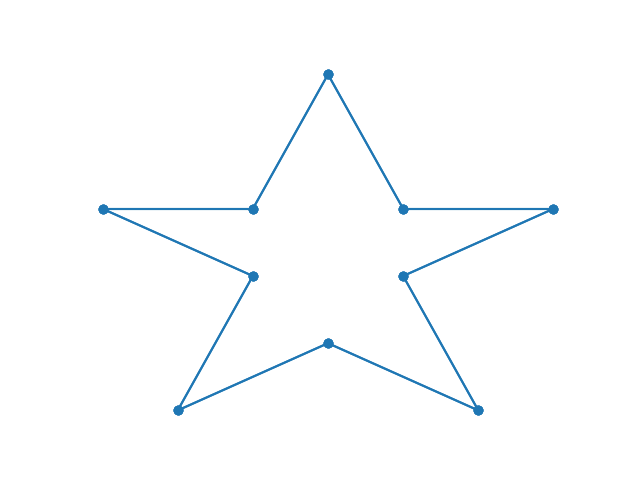
\includegraphics[width = \textwidth]{pentagram.png}
        \caption{Star test input polygon.}
        \label{fig:star}
    \end{subfigure}
    \begin{subfigure}{0.45\textwidth}
        \centering
        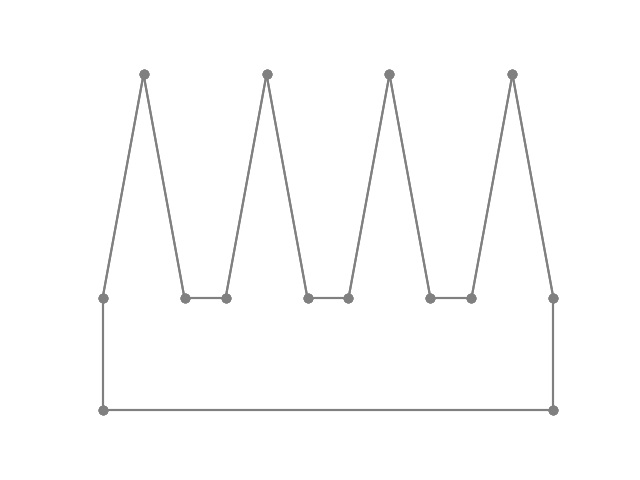
\includegraphics[width = \textwidth]{comb.png}
        \caption{Comb test input polygon.}
        \label{fig:comb}
    \end{subfigure}
    \begin{subfigure}{0.45\textwidth}
        \centering
        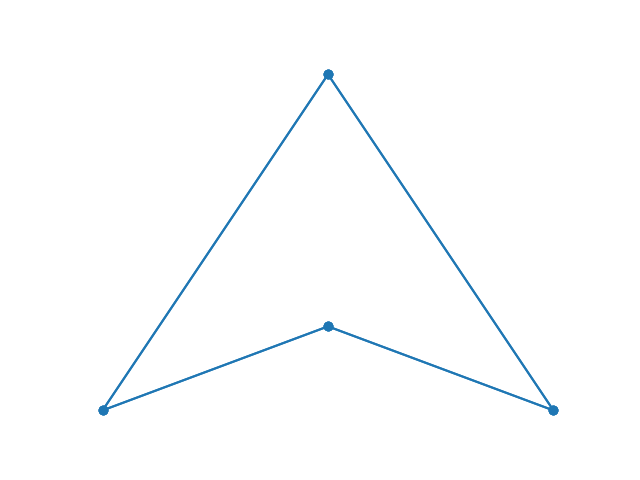
\includegraphics[width = \textwidth]{concave_triangle.png}
        \caption{Arrowhead test input polygon.}
        \label{fig:concave}
    \end{subfigure}
    \begin{subfigure}{0.45\textwidth}
        \centering
        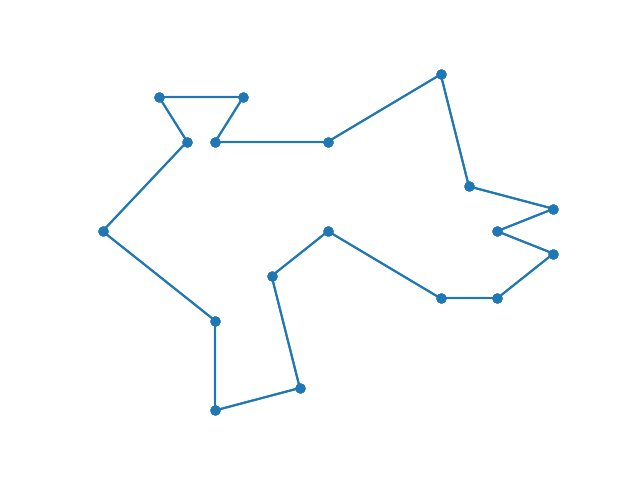
\includegraphics[width = \textwidth]{random.png}
        \caption{Arbitrary test input polygon.}
        \label{fig:random}
    \end{subfigure}
    \caption{Input polygons used for testing the algorithm.}
\end{figure}

So far:
- literature research
- created the algorithm for one guard
- implemented the gradient computation for one guard
- get multiple polygons as test cases
- have results for polygons that require rational coordinates

\subsection{Future Plans}
Future plans:
- algorithm for multiple guards
- implement algorithm for multiple guards
- test algorithm for multiple test cases 
- compare with other algorithms (error margin)